\documentclass[10pt]{extarticle}
\title{}
\author{Avinash Iyer}
\date{}

%font setup
%
%\usepackage[math]{anttor}

%paper setup
\usepackage{geometry}
\geometry{letterpaper, portrait, margin=1in}
\usepackage{fancyhdr}

%symbols
\usepackage{amsmath}
\usepackage{amssymb}
\usepackage{hyperref}
\usepackage{gensymb}

\usepackage[T1]{fontenc}
\usepackage[utf8]{inputenc}

%chemistry stuff
\usepackage[version=4]{mhchem}
\usepackage{chemfig}

%plotting
\usepackage{pgfplots}
\usepackage{tikz}

%\usepackage{natbib}

%graphics stuff
\usepackage{graphicx}
\graphicspath{ {./images/} }

%a useful command
\newcommand{\plain}[1]{\textrm{#1}}

%code stuff
%when using minted, make sure to add the -shell-escape flag
%you can use lstlisting if you don't want to use minted
%\usepackage{minted}
%\usemintedstyle{pastie}
%\newminted[javacode]{java}{frame=lines,framesep=2mm,linenos=true,fontsize=\footnotesize,tabsize=3,autogobble,}
%\newminted[cppcode]{cpp}{frame=lines,framesep=2mm,linenos=true,fontsize=\footnotesize,tabsize=3,autogobble,}

\usepackage{listings}
\usepackage{color}
\definecolor{dkgreen}{rgb}{0,0.6,0}
\definecolor{gray}{rgb}{0.5,0.5,0.5}
\definecolor{mauve}{rgb}{0.58,0,0.82}

\lstset{frame=tb,
	language=Java,
	aboveskip=3mm,
	belowskip=3mm,
	showstringspaces=false,
	columns=flexible,
	basicstyle={\small\ttfamily},
	numbers=none,
	numberstyle=\tiny\color{gray},
	keywordstyle=\color{blue},
	commentstyle=\color{dkgreen},
	stringstyle=\color{mauve},
	breaklines=true,
	breakatwhitespace=true,
	tabsize=3
}
\pagestyle{fancy}
\fancyhf{}
\rhead{Avinash Iyer, Tobias Searcy-Jorgensen}
\lhead{Lab 4: Measurement of $g$}
\begin{document}{
\section*{Abstract}
Two experiments were performed in order to exercise different techniques to find the acceleration due to gravity, $g$. The first experiment used a weight on the other end of a pulley to drag a cart along an air track. A sail was attached to the cart, and two photogates were placed along the path of the air track — the distance between the two photogates, the length of the sail of the cart, and the time recorded on each photogate were used to calculate the acceleration of the cart. After the acceleration of the cart was found, a formula was used relating the masses of the cart and the falling mass in order to calculate gravity. In the second experiment, a small cylindrical mass was used to elevate one section of the air track, creating an incline which the cart would accelerate down. A similar technique of calculation using photogate sensors yielded a value for acceleration, after which a formula that related the height of the track, the length of the track, and the length between two masses yielded a value of $g$. The acceleration found in the first experiment was $2.0 \pm 0.1$ m/s$^2$, with the corresponding value of $g = 9.5 \pm 0.6$ m/s$^2$. The acceleration found in the second experiment was $0.13 \pm 0.01$ m/s$^2$, with the corresponding value of $g = 10.4 \pm 0.9$ m/s$^2$. These results are consistent with the commonly accepted value of $g = 9.8$ m/s$^2$.
\section*{Experiment I}
\subsection*{Part 1}
\begin{quote}
	Does the set-up of the experiment have anything to do with how far away the cart begins from the first photogate?  With that in mind, is it necessary for the cart to be released from the exact same location every time?  Explain your answer in detail.  If so, be sure to start the cart from the exact same location every time.  If not, be sure to perform multiple trials from different starting points in order to evaluate the random uncertainty in the result.
\end{quote}		
No, the release point of the cart does not have an effect on the measured acceleration, as the acceleration is a function of the distance between the two photogates.
\subsection*{Part 2}
\begin{quote}
	Design and describe in detail the experiment that you will perform in order to determine gravitational acceleration.  Include a labeled sketch of the design of the experiment.  Which physical quantities must be measured and how will you measure them?
\end{quote}
[sketch here]

We will measure the masses of the cart and the falling mass, as well as the distance between the two photogates on the track's ruler.
\subsection*{Part 3}
\begin{quote}
	Give a detailed explanation of the mathematical procedures that will be followed in order to determine gravitational acceleration from the measured quantities.  Be sure to define and explain every variable that you introduce in the mathematical expression.
\end{quote}
We measure $a = \frac{\left(\frac{l}{t_1}\right)^2 - \left(\frac{l}{t_0}\right)^2}{2d}$, where $l$ is the length of the sail of the cart. Afterwards, we will use the following progression of formulae to find the gravitational acceleration. $M$ is the mass of the cart, and $m$ is the mass of the falling mass.
\begin{align*}
	T & = Ma \\
	mg - T &= ma \\
	mg - Ma &= ma \\
	g &= \frac{a(M+m)}{m}
\end{align*}
\subsection*{Part 4}
\begin{quote}
	Give a list of assumptions about the objects, interactions, and processes that need to be made in order to solve the problem, with clear explanations of how these assumptions affect the result.
\end{quote}
We are assuming that the falling mass is released with no extra push, which would increase the acceleration. On the other hand, we are also assuming zero friction — friction would decrease the measured acceleration.
\subsection*{Part 5}
\begin{quote}
	Give a list of possible sources of experimental uncertainty and a clear description of the steps that were taken to minimize the uncertainties and undesirable side effects.
\end{quote}
\begin{itemize}
	\item Instrumental uncertainties: We are using a triple beam balance, which has an instrumental uncertainty to the nearest 0.1 grams, as well as depending on a ruler with instrumental uncertainty to the nearest 0.5 mm.
	\item Random uncertainties and Problem of Definition: We will use a consistent measurement from one side of the photogate in order to reduce the random uncertainty and resolve the problem of definition problems.
\end{itemize}
\subsection*{Parts 6\textendash 8}
\begin{quote}
	(6) Perform the experiment and record the data in an organized data table. Show samples of any intermediate calculations that were performed. \\
	(7) Determine the acceleration of the cart and report it in a format appropriate for a lab report, i.e. $ a = a_{\plain{best}} \pm \delta a $.  Show all of your work. \\
	(8) Determine gravitational acceleration $ g $ along with its uncertainty and report the result in an appropriate format.  Show your work.
\end{quote}
\begin{center}
	\begin{tabular}{c|c}
		Quantity & Measurement with error \\
		\hline
		$ M $ & $190.5 \pm 0.1$ g\\
		$ m $ & $50.4 \pm 0.1$ g \\
		$d$ & $0.70 \pm 0.01$ m  \\
		$l$ & $10.0 \pm 0.1$ cm \\
		\hline
		$t_{01}$ & $0.103 \pm 0.001$ s \\
		$t_{11}$ & $0.051 \pm 0.001$ s \\
		$t_{02}$ & $0.104 \pm 0.001$ s \\
		$t_{12}$ & $0.052 \pm 0.001$ s\\
		$t_{03}$ & $0.105 \pm 0.001$ s \\
		$t_{13}$ & $0.052 \pm 0.001$ s \\
		$t_{04}$ & $0.105 \pm 0.001$ s\\
		$t_{14}$ & $0.052 \pm 0.001$ s \\
		$t_{05}$ & $0.105 \pm 0.001$ s \\
		$t_{15}$ & $0.053 \pm 0.001$ s  
	\end{tabular}
\end{center}
Sample calculation for first set of values (the ones denoted $t_{01}$ and $t_{11}$)is below (these values were rounded for the simplicity of display, but more precise versions were used in the Excel spreadsheet):
\begin{align*}
	v_1 &= \frac{l}{t_1} \\
	&= 1.96~\plain{m/s} \\
	\delta v_1 &= v_1\sqrt{\left(\frac{\delta t_1}{t_1}\right)^2 + \left(\frac{\delta l}{l}\right)^2} \\
	&= 0.04 \\
	v_0 &= \frac{l}{t_0} \\
	&= 0.97~\plain{m/s} \\
	\delta v_0 &= v_0\sqrt{\left(\frac{\delta t_0}{t_0}\right)^2 + \left(\frac{\delta l}{l}\right)^2} \\
	&= 0.01 \\
	v_1^2 &= 3.84~\plain{m/s} \\
	v_0^2 &= 0.94~\plain{m/s} \\
	\delta \left(v_1^2\right) &= 2v_1\delta v_1 \\
	&= 0.2 \\
	\delta \left(v_0^2\right) &= 2v_0\delta v_0 \\
	&= 0.03 \\
	v_1^2-v_0^2 &= 2.9 \\
	\delta(v_1^2-v_0^2) &= \sqrt{\left(\delta v_0^2\right)^2 + \left(\delta v_1^2\right)^2} \\
	&= 0.2 \\
	a &= \frac{v_1^2-v_0^2}{2d} \\
	&= 2.08~\plain{m/s$^2$} \\
	\delta a &= a\sqrt{\left(\frac{\delta(v_1^2-v_0^2)}{v_1^2-v_0^2}\right)^2 + \left(\frac{2\delta d}{2d}\right)^2} \\
	&= 0.1 \\
	M+m &= 240.9 \\
	\delta (M+m) &= \sqrt{(\delta m)^2 + (\delta M)^2} \\
	&= 0.1 \\
	a(M+m) &= 499 \\
	\delta(a(m+M)) &= a(M+m)\sqrt{\left(\frac{\delta a}{a}\right)^2 + \left(\frac{\delta(m+M)}{m+M}\right)^2} \\
	&= 29 \\
	g &= \frac{a(M+m)}{m} \\
	&= 9.91~\plain{m/s$^2$} \\
	\delta g &= g\sqrt{\left(\frac{\delta(a(M+m))}{a(M+m)}\right)^2 + \left(\frac{\delta m}{m}\right)} \\
	&= 0.6
 \end{align*}
The table of $a$ and $g$ values with uncertainties with results from each trial is below:
\begin{center}
	\begin{tabular}{c|c}
		Trial No. & $a \pm \delta a$ (m/s$^2$) \\
		\hline
		1 & $2.1 \pm 0.1$ \\
		2 & $2.0 \pm 0.1$ \\
		3 & $2.0 \pm 0.1$ \\
		4 & $2.0 \pm 0.1$ \\
		5 & $1.9 \pm 0.1$
	\end{tabular}
	\begin{tabular}{c|c}
		Trial No. & $g \pm \delta g$ (m/s$^2$)\\
		\hline
		1 & $9.9\pm 0.6$ \\
		2 & $9.5 \pm 0.6$ \\
		3 & $9.5 \pm 0.6$ \\
		4 & $9.5\pm 0.6$ \\
		5 & $9.1 \pm 0.5$
	\end{tabular}
\end{center}
Using error propagation rules, we find the final values for $a$ and $g$ below:
\begin{align*}
	a &= 2.0 \pm 0.1~\plain{m/s$^2$} \\
	g &= 9.5 \pm 0.6~\plain{m/s$^{2}$}
\end{align*}
\section*{Experiment II}
\begin{quote}
	Design another experiment to determine gravitational acceleration.  This new experiment must utilize a different method to measure acceleration of the cart.
\end{quote}
\subsection*{Part 1}
\begin{quote}
	Design and describe in detail the experiment that you will perform in order to determine gravitational acceleration.  Include a labeled sketch of the design of the experiment.  Which physical quantities must be measured and how will you measure them?
\end{quote}
We propped the track up on an incline and placed our two photogates $0.70$ meters apart from each other. We then release the cart without pushing it, and let it slide down the track along the two photgates. We will use the velocities calculate from the photogates in a similar manner to the previous experiment, as well as the horizontal distance between the two points, in order to find the final value of $a$, and therefore $g$.\\
\\
A picture depicting the experimental setup is shown below (not to scale). Included are the measured distances and their errors. The total distance $x$ of the track is $1.00 \pm 0.01$ m.
\begin{center}
	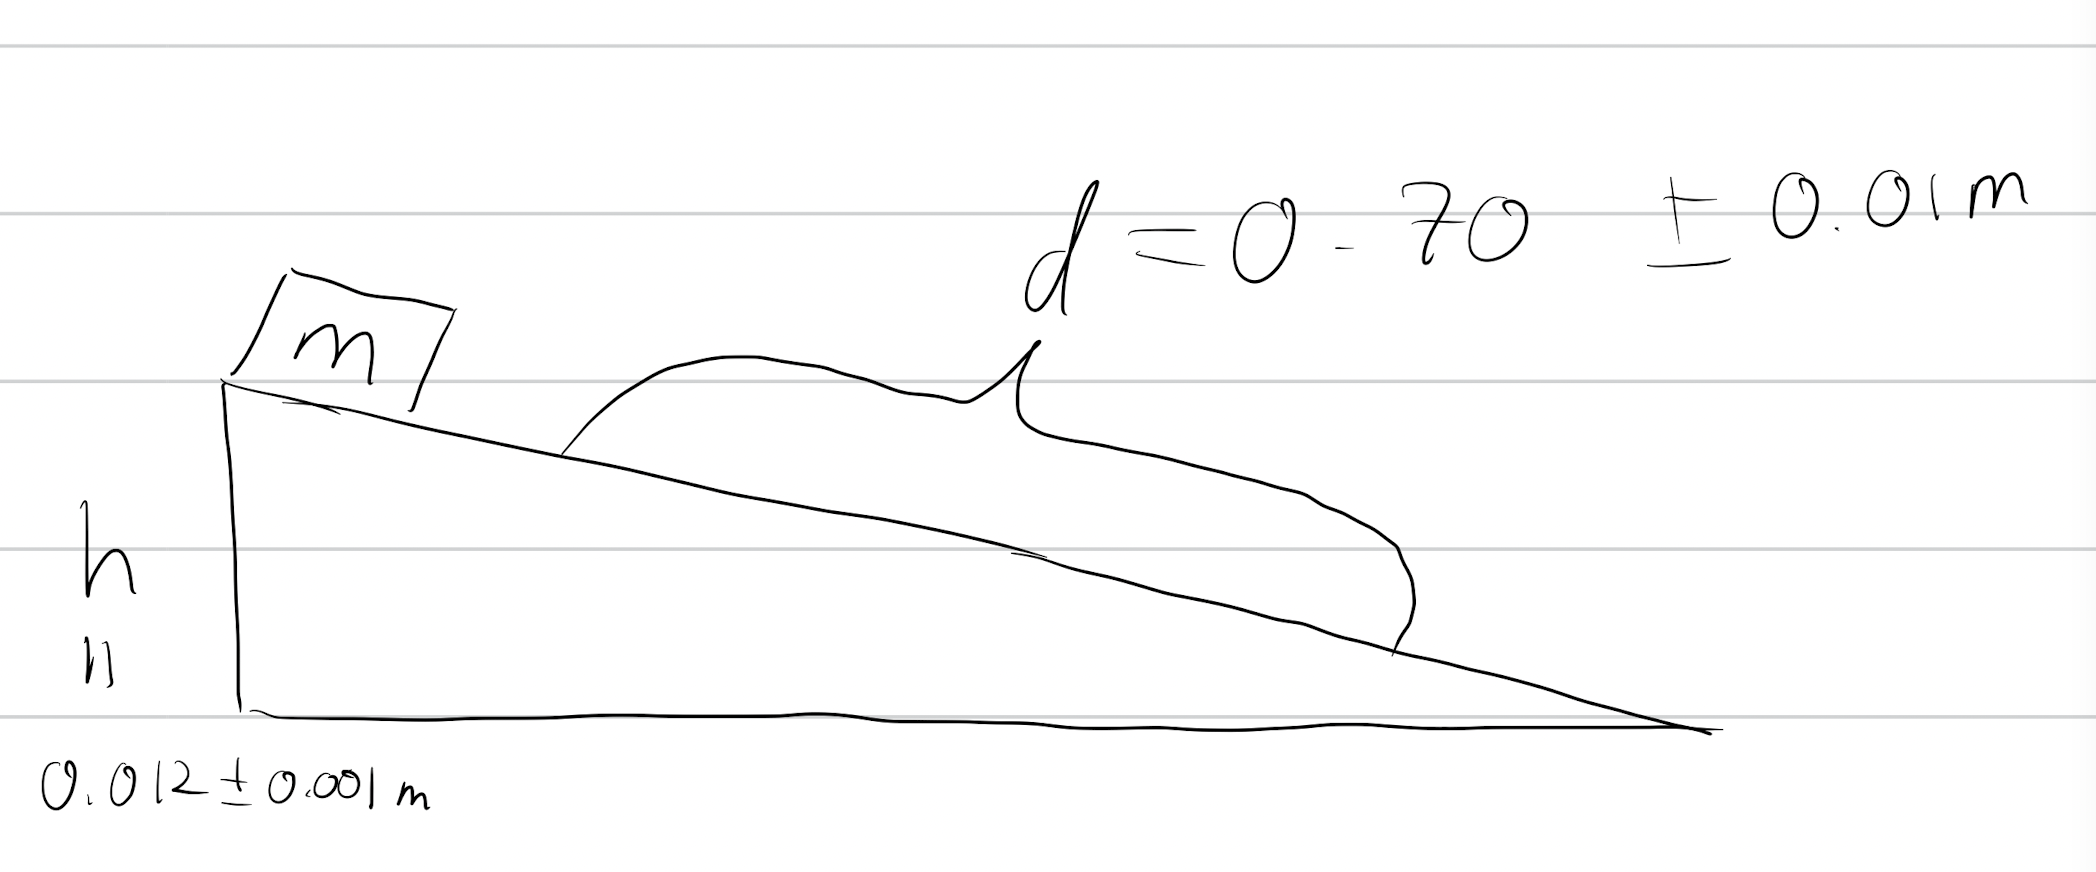
\includegraphics[width=10cm]{Lab4Image2_1}
\end{center}
\subsection*{Part 2}
The primary source of experimental error is the way we measured height, as we did not use a set of vernier calipers. We were able to minimize error everywhere else, but even then, our measurement for $h$ had an approximately $8.3\%$ error.
\subsection*{Part 3}
Because the experimental error for $h$ was nearly an order of magnitude higher than the experimental error for $d$ or $l$ (the length of the cart's sail), we did not use error propagation to find the value of $a$ or $g$ and just utilized the fractional error to calculate our final absolute error.
\begin{center}
	\begin{tabular}{c|c}
		Quantity & Measurement with Error \\
		\hline
		$h$ & $0.012\pm 0.001$ m\\
		$d$ & $0.70 \pm 0.01$ m \\
		$l$ & $0.100 \pm 0.001$ m \\
		$x$ & $1.00 \pm 0.01$ m \\
		\hline
		$t_{01}$ & $0.226 \pm 0.001$ s \\
		$t_{11}$ & $0.164 \pm 0.001$ s \\
		$t_{02}$ & $0.225 \pm 0.001$ s \\
		$t_{12}$ & $0.164 \pm 0.001$ s \\
		$t_{03}$ & $0.224 \pm 0.001$ s \\
		$t_{13}$ & $0.163 \pm 0.001$ s \\
		$t_{04}$ & $0.225 \pm 0.001$ s \\
		$t_{14}$ & $0.164 \pm 0.001$ s \\
		$t_{05}$ & $0.225 \pm 0.001$ s \\
		$t_{15}$ & $0.163 \pm 0.001$ s
	\end{tabular}
\end{center}
\subsection*{Part 4}
\begin{quote}
	Determine the acceleration of the cart and report it in an appropriate format.
\end{quote}
We calculate $a$ for the first value, and from there we apply our error propagation of $8.3\%$.
\begin{align*}
	a &= \frac{\left(\frac{l}{t_{11}}\right)^2 - \left(\frac{l}{t_{01}}\right)^2}{2d} \\
	&= 0.13\pm 0.01~\plain{m/s$^{2}$} \\
\end{align*}
\subsection*{Part 5}
\begin{quote}
	Determine gravitational acceleration and report the result in an appropriate format. Show your work.
\end{quote}
\begin{align*}
	g &= \frac{a}{\sin \theta} \\
	&= \frac{a}{\frac{h}{\sqrt{h^2 + x^2}}} \\
	&= 10.4 \pm 0.9 ~\plain{m/s$^{2}$}
\end{align*}
\pagebreak
\section*{Conclusion}
\subsection*{Part 1}
\begin{quote}
	Are the two values that you obtained for gravitational acceleration consistent with each other?  If not, discuss possible reasons.
\end{quote}
Yes, our two values for gravitational acceleration are consistent with each other.
\subsection*{Part 2}
\begin{quote}
	Which of these two results is more precise?  How do you know? Show your calculations.
\end{quote}
Our first result yields a fractional uncertainty of $\frac{\delta g}{g} = 6\%$, while our second result yields a fractional uncertainty of $8.3\%$, so our first result is more precise.
\subsection*{Part 3}
\begin{quote}
	Are the experimental values of gravitational acceleration consistent with the accepted value? 
\end{quote}
Yes, our experimental values are consistent with the accepted value.
\subsection*{Part 4}
\begin{quote}
	Are the experimental values larger or smaller than the theoretical value? What effect could your assumptions have had on the experimental values?
\end{quote}
Our experimental value for the first experiment is smaller than the theoretical value, which is likely due to our assumption of zero friction having been false. Meanwhile, our second experimental value was higher than the theoretical value, which is likely because our measured value of $h$ was lower than the actual value of $h$.
}\end{document}
